% Created by tikzDevice version 0.6.2-92-0ad2792 on 2012-09-16 00:29:07
% !TEX encoding = UTF-8 Unicode
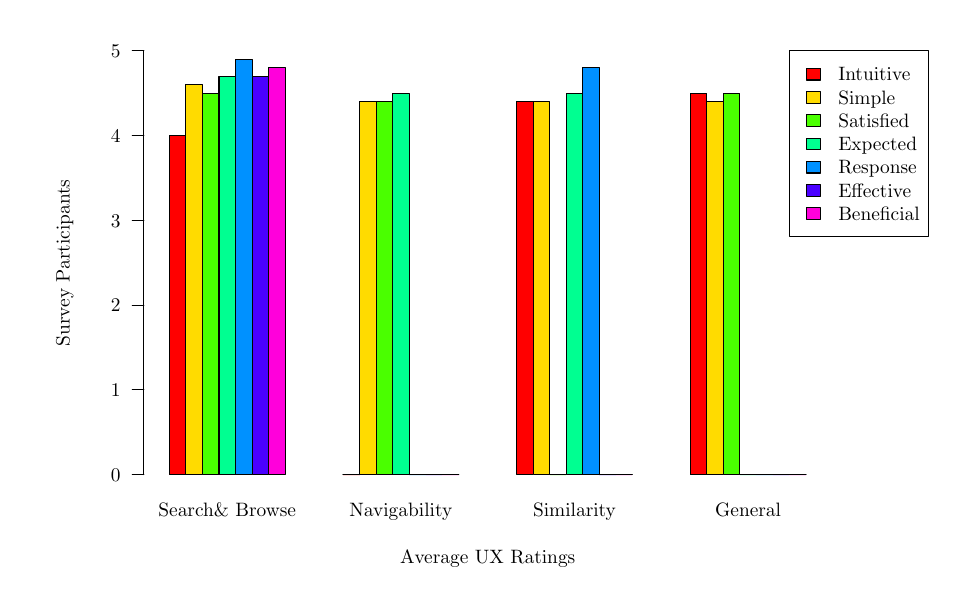
\begin{tikzpicture}[x=1pt,y=1pt]
\definecolor[named]{fillColor}{rgb}{1.00,1.00,1.00}
\path[use as bounding box,fill=fillColor,fill opacity=0.00] (0,0) rectangle (332.44,195.13);
\begin{scope}
\path[clip] (  0.00,  0.00) rectangle (332.44,195.13);
\definecolor[named]{drawColor}{rgb}{0.00,0.00,0.00}
\definecolor[named]{fillColor}{rgb}{1.00,0.00,0.00}

\path[draw=drawColor,line width= 0.4pt,line join=round,line cap=round,fill=fillColor] ( 51.20, 33.60) rectangle ( 57.18,156.10);
\definecolor[named]{fillColor}{rgb}{1.00,0.86,0.00}

\path[draw=drawColor,line width= 0.4pt,line join=round,line cap=round,fill=fillColor] ( 57.18, 33.60) rectangle ( 63.15,174.48);
\definecolor[named]{fillColor}{rgb}{0.29,1.00,0.00}

\path[draw=drawColor,line width= 0.4pt,line join=round,line cap=round,fill=fillColor] ( 63.15, 33.60) rectangle ( 69.13,171.42);
\definecolor[named]{fillColor}{rgb}{0.00,1.00,0.57}

\path[draw=drawColor,line width= 0.4pt,line join=round,line cap=round,fill=fillColor] ( 69.13, 33.60) rectangle ( 75.10,177.54);
\definecolor[named]{fillColor}{rgb}{0.00,0.57,1.00}

\path[draw=drawColor,line width= 0.4pt,line join=round,line cap=round,fill=fillColor] ( 75.10, 33.60) rectangle ( 81.08,183.67);
\definecolor[named]{fillColor}{rgb}{0.29,0.00,1.00}

\path[draw=drawColor,line width= 0.4pt,line join=round,line cap=round,fill=fillColor] ( 81.08, 33.60) rectangle ( 87.05,177.54);
\definecolor[named]{fillColor}{rgb}{1.00,0.00,0.86}

\path[draw=drawColor,line width= 0.4pt,line join=round,line cap=round,fill=fillColor] ( 87.05, 33.60) rectangle ( 93.03,180.60);
\definecolor[named]{fillColor}{rgb}{1.00,0.00,0.00}

\path[draw=drawColor,line width= 0.4pt,line join=round,line cap=round,fill=fillColor] (113.94, 33.60) rectangle (119.91, 33.60);
\definecolor[named]{fillColor}{rgb}{1.00,0.86,0.00}

\path[draw=drawColor,line width= 0.4pt,line join=round,line cap=round,fill=fillColor] (119.91, 33.60) rectangle (125.89,168.35);
\definecolor[named]{fillColor}{rgb}{0.29,1.00,0.00}

\path[draw=drawColor,line width= 0.4pt,line join=round,line cap=round,fill=fillColor] (125.89, 33.60) rectangle (131.86,168.35);
\definecolor[named]{fillColor}{rgb}{0.00,1.00,0.57}

\path[draw=drawColor,line width= 0.4pt,line join=round,line cap=round,fill=fillColor] (131.86, 33.60) rectangle (137.84,171.42);
\definecolor[named]{fillColor}{rgb}{0.00,0.57,1.00}

\path[draw=drawColor,line width= 0.4pt,line join=round,line cap=round,fill=fillColor] (137.84, 33.60) rectangle (143.81, 33.60);
\definecolor[named]{fillColor}{rgb}{0.29,0.00,1.00}

\path[draw=drawColor,line width= 0.4pt,line join=round,line cap=round,fill=fillColor] (143.81, 33.60) rectangle (149.79, 33.60);
\definecolor[named]{fillColor}{rgb}{1.00,0.00,0.86}

\path[draw=drawColor,line width= 0.4pt,line join=round,line cap=round,fill=fillColor] (149.79, 33.60) rectangle (155.76, 33.60);
\definecolor[named]{fillColor}{rgb}{1.00,0.00,0.00}

\path[draw=drawColor,line width= 0.4pt,line join=round,line cap=round,fill=fillColor] (176.68, 33.60) rectangle (182.65,168.35);
\definecolor[named]{fillColor}{rgb}{1.00,0.86,0.00}

\path[draw=drawColor,line width= 0.4pt,line join=round,line cap=round,fill=fillColor] (182.65, 33.60) rectangle (188.63,168.35);
\definecolor[named]{fillColor}{rgb}{0.29,1.00,0.00}

\path[draw=drawColor,line width= 0.4pt,line join=round,line cap=round,fill=fillColor] (188.63, 33.60) rectangle (194.60, 33.60);
\definecolor[named]{fillColor}{rgb}{0.00,1.00,0.57}

\path[draw=drawColor,line width= 0.4pt,line join=round,line cap=round,fill=fillColor] (194.60, 33.60) rectangle (200.58,171.42);
\definecolor[named]{fillColor}{rgb}{0.00,0.57,1.00}

\path[draw=drawColor,line width= 0.4pt,line join=round,line cap=round,fill=fillColor] (200.58, 33.60) rectangle (206.55,180.60);
\definecolor[named]{fillColor}{rgb}{0.29,0.00,1.00}

\path[draw=drawColor,line width= 0.4pt,line join=round,line cap=round,fill=fillColor] (206.55, 33.60) rectangle (212.53, 33.60);
\definecolor[named]{fillColor}{rgb}{1.00,0.00,0.86}

\path[draw=drawColor,line width= 0.4pt,line join=round,line cap=round,fill=fillColor] (212.53, 33.60) rectangle (218.50, 33.60);
\definecolor[named]{fillColor}{rgb}{1.00,0.00,0.00}

\path[draw=drawColor,line width= 0.4pt,line join=round,line cap=round,fill=fillColor] (239.42, 33.60) rectangle (245.39,171.42);
\definecolor[named]{fillColor}{rgb}{1.00,0.86,0.00}

\path[draw=drawColor,line width= 0.4pt,line join=round,line cap=round,fill=fillColor] (245.39, 33.60) rectangle (251.37,168.35);
\definecolor[named]{fillColor}{rgb}{0.29,1.00,0.00}

\path[draw=drawColor,line width= 0.4pt,line join=round,line cap=round,fill=fillColor] (251.37, 33.60) rectangle (257.34,171.42);
\definecolor[named]{fillColor}{rgb}{0.00,1.00,0.57}

\path[draw=drawColor,line width= 0.4pt,line join=round,line cap=round,fill=fillColor] (257.34, 33.60) rectangle (263.32, 33.60);
\definecolor[named]{fillColor}{rgb}{0.00,0.57,1.00}

\path[draw=drawColor,line width= 0.4pt,line join=round,line cap=round,fill=fillColor] (263.32, 33.60) rectangle (269.29, 33.60);
\definecolor[named]{fillColor}{rgb}{0.29,0.00,1.00}

\path[draw=drawColor,line width= 0.4pt,line join=round,line cap=round,fill=fillColor] (269.29, 33.60) rectangle (275.27, 33.60);
\definecolor[named]{fillColor}{rgb}{1.00,0.00,0.86}

\path[draw=drawColor,line width= 0.4pt,line join=round,line cap=round,fill=fillColor] (275.27, 33.60) rectangle (281.24, 33.60);
\end{scope}
\begin{scope}
\path[clip] (  0.00,  0.00) rectangle (332.44,195.13);
\definecolor[named]{drawColor}{rgb}{0.00,0.00,0.00}

\node[text=drawColor,anchor=base,inner sep=0pt, outer sep=0pt, scale=  0.70] at ( 72.11, 18.48) {Search\& Browse};

\node[text=drawColor,anchor=base,inner sep=0pt, outer sep=0pt, scale=  0.70] at (134.85, 18.48) {Navigability};

\node[text=drawColor,anchor=base,inner sep=0pt, outer sep=0pt, scale=  0.70] at (197.59, 18.48) {Similarity};

\node[text=drawColor,anchor=base,inner sep=0pt, outer sep=0pt, scale=  0.70] at (260.33, 18.48) {General};
\end{scope}
\begin{scope}
\path[clip] (  0.00,  0.00) rectangle (332.44,195.13);
\definecolor[named]{drawColor}{rgb}{0.00,0.00,0.00}

\node[text=drawColor,anchor=base,inner sep=0pt, outer sep=0pt, scale=  0.70] at (166.22,  1.68) {Average UX Ratings};

\node[text=drawColor,rotate= 90.00,anchor=base,inner sep=0pt, outer sep=0pt, scale=  0.70] at ( 15.12,110.16) {Survey Participants};
\end{scope}
\begin{scope}
\path[clip] (  0.00,  0.00) rectangle (332.44,195.13);
\definecolor[named]{drawColor}{rgb}{0.00,0.00,0.00}

\path[draw=drawColor,line width= 0.4pt,line join=round,line cap=round] ( 42.00, 33.60) -- ( 42.00,186.73);

\path[draw=drawColor,line width= 0.4pt,line join=round,line cap=round] ( 42.00, 33.60) -- ( 37.80, 33.60);

\path[draw=drawColor,line width= 0.4pt,line join=round,line cap=round] ( 42.00, 64.23) -- ( 37.80, 64.23);

\path[draw=drawColor,line width= 0.4pt,line join=round,line cap=round] ( 42.00, 94.85) -- ( 37.80, 94.85);

\path[draw=drawColor,line width= 0.4pt,line join=round,line cap=round] ( 42.00,125.48) -- ( 37.80,125.48);

\path[draw=drawColor,line width= 0.4pt,line join=round,line cap=round] ( 42.00,156.10) -- ( 37.80,156.10);

\path[draw=drawColor,line width= 0.4pt,line join=round,line cap=round] ( 42.00,186.73) -- ( 37.80,186.73);

\node[text=drawColor,anchor=base east,inner sep=0pt, outer sep=0pt, scale=  0.70] at ( 33.60, 31.19) {0};

\node[text=drawColor,anchor=base east,inner sep=0pt, outer sep=0pt, scale=  0.70] at ( 33.60, 61.82) {1};

\node[text=drawColor,anchor=base east,inner sep=0pt, outer sep=0pt, scale=  0.70] at ( 33.60, 92.44) {2};

\node[text=drawColor,anchor=base east,inner sep=0pt, outer sep=0pt, scale=  0.70] at ( 33.60,123.07) {3};

\node[text=drawColor,anchor=base east,inner sep=0pt, outer sep=0pt, scale=  0.70] at ( 33.60,153.69) {4};

\node[text=drawColor,anchor=base east,inner sep=0pt, outer sep=0pt, scale=  0.70] at ( 33.60,184.32) {5};
\end{scope}
\begin{scope}
\path[clip] (  0.00,  0.00) rectangle (332.44,195.13);
\definecolor[named]{drawColor}{rgb}{0.00,0.00,0.00}

\path[draw=drawColor,line width= 0.4pt,line join=round,line cap=round] (275.27,186.73) rectangle (325.51,119.53);
\definecolor[named]{fillColor}{rgb}{1.00,0.00,0.00}

\path[draw=drawColor,line width= 0.4pt,line join=round,line cap=round,fill=fillColor] (281.57,180.43) rectangle (286.61,176.23);
\definecolor[named]{fillColor}{rgb}{1.00,0.86,0.00}

\path[draw=drawColor,line width= 0.4pt,line join=round,line cap=round,fill=fillColor] (281.57,172.03) rectangle (286.61,167.83);
\definecolor[named]{fillColor}{rgb}{0.29,1.00,0.00}

\path[draw=drawColor,line width= 0.4pt,line join=round,line cap=round,fill=fillColor] (281.57,163.63) rectangle (286.61,159.43);
\definecolor[named]{fillColor}{rgb}{0.00,1.00,0.57}

\path[draw=drawColor,line width= 0.4pt,line join=round,line cap=round,fill=fillColor] (281.57,155.23) rectangle (286.61,151.03);
\definecolor[named]{fillColor}{rgb}{0.00,0.57,1.00}

\path[draw=drawColor,line width= 0.4pt,line join=round,line cap=round,fill=fillColor] (281.57,146.83) rectangle (286.61,142.63);
\definecolor[named]{fillColor}{rgb}{0.29,0.00,1.00}

\path[draw=drawColor,line width= 0.4pt,line join=round,line cap=round,fill=fillColor] (281.57,138.43) rectangle (286.61,134.23);
\definecolor[named]{fillColor}{rgb}{1.00,0.00,0.86}

\path[draw=drawColor,line width= 0.4pt,line join=round,line cap=round,fill=fillColor] (281.57,130.03) rectangle (286.61,125.83);

\node[text=drawColor,anchor=base west,inner sep=0pt, outer sep=0pt, scale=  0.70] at (292.91,175.92) {Intuitive};

\node[text=drawColor,anchor=base west,inner sep=0pt, outer sep=0pt, scale=  0.70] at (292.91,167.52) {Simple};

\node[text=drawColor,anchor=base west,inner sep=0pt, outer sep=0pt, scale=  0.70] at (292.91,159.12) {Satisfied};

\node[text=drawColor,anchor=base west,inner sep=0pt, outer sep=0pt, scale=  0.70] at (292.91,150.72) {Expected};

\node[text=drawColor,anchor=base west,inner sep=0pt, outer sep=0pt, scale=  0.70] at (292.91,142.32) {Response};

\node[text=drawColor,anchor=base west,inner sep=0pt, outer sep=0pt, scale=  0.70] at (292.91,133.92) {Effective};

\node[text=drawColor,anchor=base west,inner sep=0pt, outer sep=0pt, scale=  0.70] at (292.91,125.52) {Beneficial};
\end{scope}
\end{tikzpicture}
